\begin{figure}[t]
\uwsinglespace
\begin{center}
\begin{minipage}{0.45\textwidth}
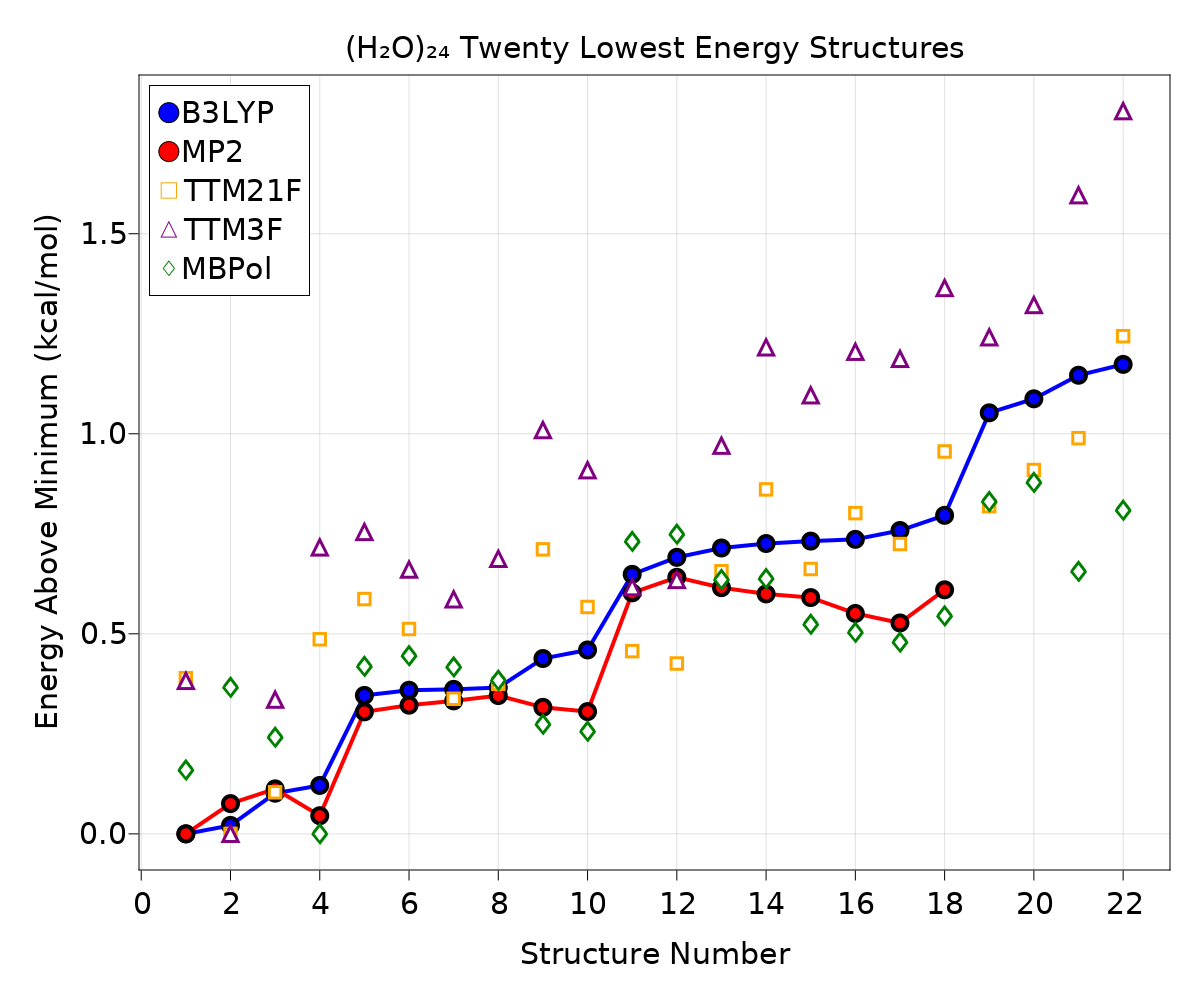
\includegraphics[width=\textwidth]{Figures/Chapter_6/w24_lowest_22_dipole_structures.png}
\end{minipage}
\begin{minipage}{0.45\textwidth}
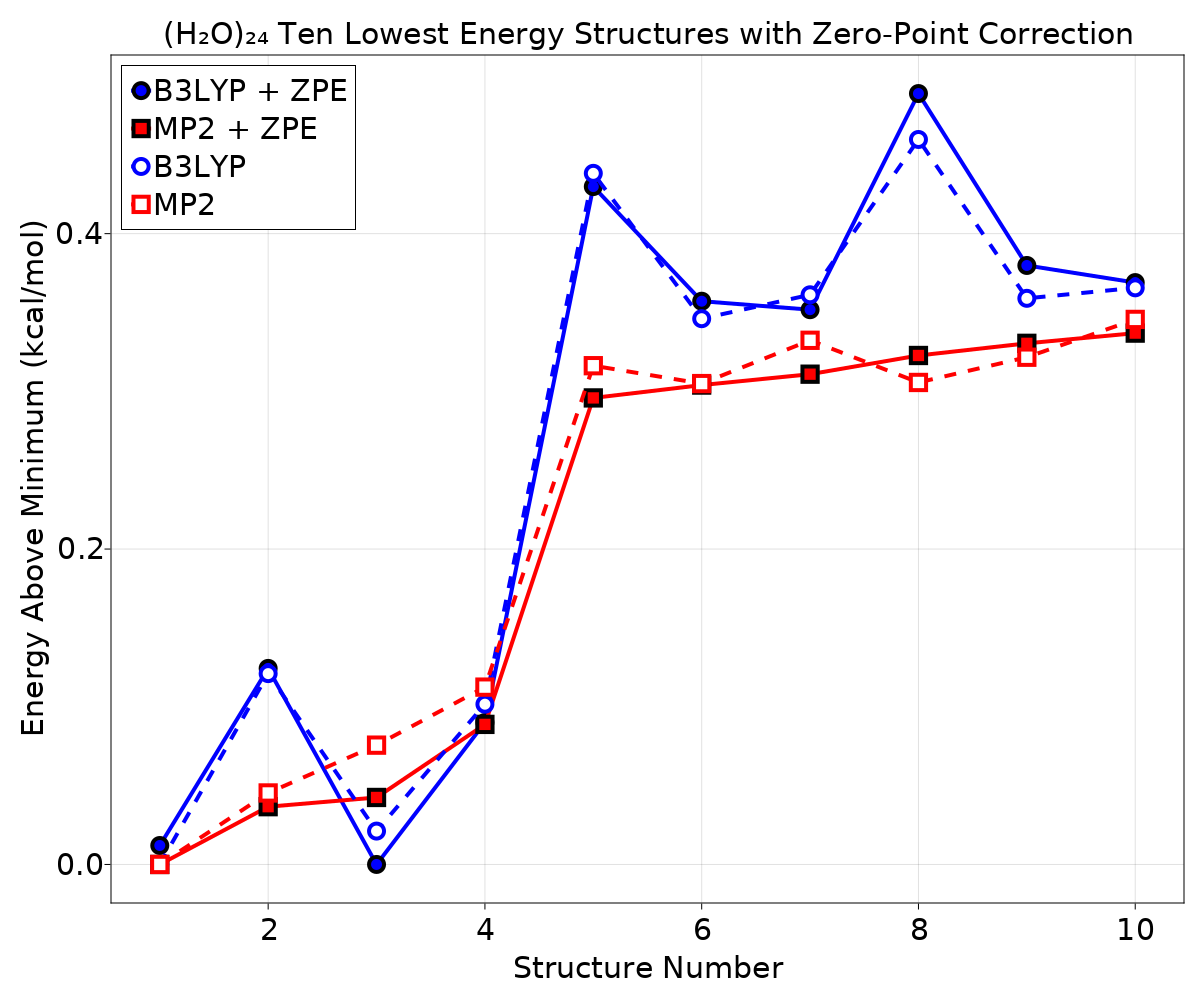
\includegraphics[width=\textwidth]{Figures/Chapter_6/w24_lowest_ten_structures_plus_zpe.png}
\end{minipage}
\end{center}
\begin{spacing}{1.0}
\caption[The left panel shows a comparison of B3LYP/TZVP and MP2/TZVP calculations of the 22 lowest \ce{(H2O)_{24}} structures with minimal dipoles. Calculations with TTM2.1-F, TTM3-F, and MB-Pol are also shown. The right panel shows the effect of harmonic zero-point energy correction on these ten lowest structures.]{The left panel shows a comparison of B3LYP/TZVP and MP2/TZVP calculations of the 22 lowest \ce{(H2O)_{24}} structures with minimal dipoles. Calculations with TTM2.1-F, TTM3-F, and MB-Pol are also shown. The right panel shows the effect of harmonic zero-point energy correction on these ten lowest structures.}\label{fig:MBE_III_F6}
\end{spacing}
\end{figure}